\chapter{What lm8-gcc do}
Xilinx有8位的PicoBlaze处理器,Lattice也有一个8位的处理器Mico8。
以下是PicoBlaze的系统框架图\footnote{图片来自PicoBlaze Manual.pdf,Page8} \\
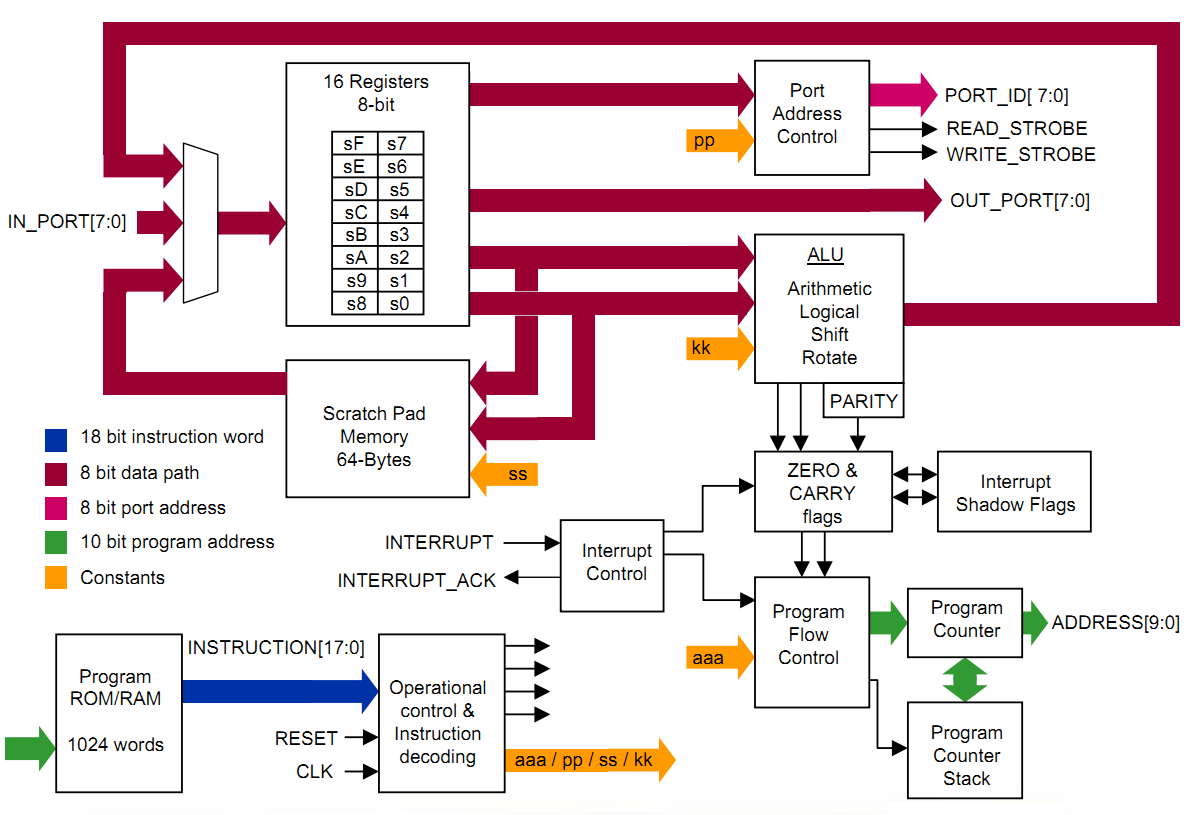
\includegraphics[width=\textwidth]{pb8arch}

这个是Mico8的系统框架图\footnote{图片来自rd1026.pdf,Page1} \\
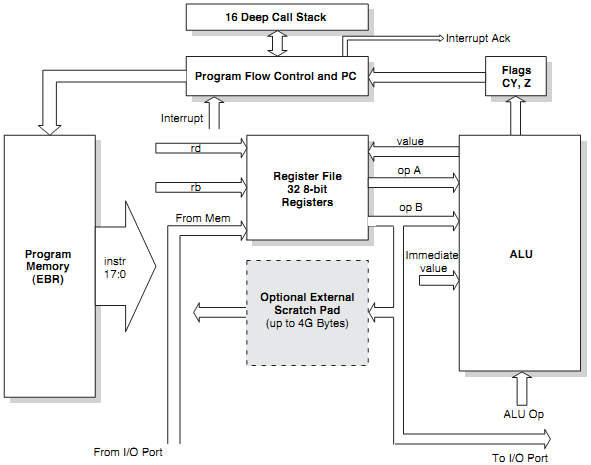
\includegraphics[width=\textwidth]{lm8arch}

仔细看系统框图,发觉Mico8和PicoBlaze的设计很相似。
更让人惊喜的是Lattice已经移植了Mico8版本的GCC,这样意味着很有可能把这个
GCC修改一下支持PicoBlaze!
也可以学习移植GCC,毕竟gcc的x86、arm、sparc都不简单。

\clearpage
\section{Compare}
既然要想弄明白Lattice是怎么移植GCC的,那么最好的办法就是
找出lm8-gcc和原始的gcc之间的差异,然后对比差异来学习。

这么一来第一件事就是找到两份源代码,一个是lm8-gcc,另一个是原始的gcc。
在Lattice找到了LatticeMico8\_Tools\_v3\_15的链接,
下载回来是 gcc-lm8-2010-09-28.tar.bz2,这个就是移植Mico8的gcc。
解压后可以知道这个gcc-lm8是以GCC 4.4.3为基础改出来的。
那么我们再到GCC的ftp把 gcc-4.4.3.tar.bz2 下载回来。

我把lm8-gcc的源码解压为gcc-4.4.3-lm8,把原始的gcc解压为gcc-4.4.3-org。
需要对比差异,最简单的就是使用diff工具,在linux下这个工具常用来生成patch文件。

至于diff怎么用,直接输入以下命令:
\begin{shcode}
#/bin/sh
diff --help
\end{shcode}

输出如下:
\begin{textcode}
Usage: diff [OPTION]... FILE1 FILE2

  -i  --ignore-case  Consider upper- and lower-case to be the same.
  -w  --ignore-all-space  Ignore all white space.
  -b  --ignore-space-change  Ignore changes in the amount of white space.
  -B  --ignore-blank-lines  Ignore changes whose lines are all blank.
  -I RE  --ignore-matching-lines=RE  Ignore changes whose lines all match RE.
  --binary  Read and write data in binary mode.
  -a  --text  Treat all files as text.

  -c  -C NUM  --context[=NUM]  Output NUM (default 2) lines of copied context.
  -u  -U NUM  --unified[=NUM]  Output NUM (default 2) lines of unified context.
    -NUM  Use NUM context lines.
    -L LABEL  --label LABEL  Use LABEL instead of file name.
    -p  --show-c-function  Show which C function each change is in.
    -F RE  --show-function-line=RE  Show the most recent line matching RE.
  -q  --brief  Output only whether files differ.
  -e  --ed  Output an ed script.
  -n  --rcs  Output an RCS format diff.
  -y  --side-by-side  Output in two columns.
    -w NUM  --width=NUM  Output at most NUM (default 130) characters per line.
    --left-column  Output only the left column of common lines.
    --suppress-common-lines  Do not output common lines.
  -DNAME  --ifdef=NAME  Output merged file to show `#ifdef NAME' diffs.
  --GTYPE-group-format=GFMT  Similar, but format GTYPE input groups with GFMT.
  --line-format=LFMT  Similar, but format all input lines with LFMT.
  --LTYPE-line-format=LFMT  Similar, but format LTYPE input lines with LFMT.
    LTYPE is `old', `new', or `unchanged'.  GTYPE is LTYPE or `changed'.
    GFMT may contain:
      %<  lines from FILE1
      %>  lines from FILE2
      %=  lines common to FILE1 and FILE2
      %[-][WIDTH][.[PREC]]{doxX}LETTER  printf-style spec for LETTER
        LETTERs are as follows for new group, lower case for old group:
          F  first line number
          L  last line number
          N  number of lines = L-F+1
          E  F-1
          M  L+1
    LFMT may contain:
      %L  contents of line
      %l  contents of line, excluding any trailing newline
      %[-][WIDTH][.[PREC]]{doxX}n  printf-style spec for input line number
    Either GFMT or LFMT may contain:
      %%  %
      %c'C'  the single character C
      %c'\OOO'  the character with octal code OOO

  -l  --paginate  Pass the output through `pr' to paginate it.
  -t  --expand-tabs  Expand tabs to spaces in output.
  -T  --initial-tab  Make tabs line up by prepending a tab.

  -r  --recursive  Recursively compare any subdirectories found.
  -N  --new-file  Treat absent files as empty.
  -P  --unidirectional-new-file  Treat absent first files as empty.
  -s  --report-identical-files  Report when two files are the same.
  -x PAT  --exclude=PAT  Exclude files that match PAT.
  -X FILE  --exclude-from=FILE  Exclude files that match any pattern in FILE.
  -S FILE  --starting-file=FILE  Start with FILE when comparing directories.

  --horizon-lines=NUM  Keep NUM lines of the common prefix and suffix.
  -d  --minimal  Try hard to find a smaller set of changes.
  -H  --speed-large-files  Assume large files and many scattered small changes.

  -v  --version  Output version info.
  --help  Output this help.

If FILE1 or FILE2 is `-', read standard input.
\end{textcode}

这个说明是很详细的,基本上不用再多说什么了。

我使用以下的命令对比。参数u是添加行号;N是如果文件是新增的,那么把源文件当成空的;r是递归调用。
(由于GCC源码太大,对比的时间很长,耐心等候吧)
\begin{shcode}
#/bin/sh
diff -uNr gcc-4.4.3-org gcc-4.4.3-lm8 > result.diff
\end{shcode}

得到差异结果有130Kb,不方便阅读,也不方便贴出来,所以自己写个简单的python脚本提取文件名。
这样就相当于有了一个索引,阅读和定位都方便很多。

\textbf{diffbrief.py}
\begin{pythoncode}
#!/bin/python
import sys, re

fin = open(sys.argv[1])
lines = fin.read()
fin.close()

regex_prefix = re.compile(r'^diff -uNr ')
regex_header = re.compile(r'^diff -uNr ([^ ]+) ([^ ]+)')
lineno = 1

for line in lines.split('\n'):
    if regex_prefix.match(line):
        res = regex_header.search(line)
        relative_path = res.groups()[0]
        relative_path = '/'.join(relative_path.split('\\')[1:])
        print '%04d: %s' % (lineno, relative_path)
    lineno += 1
\end{pythoncode}



输出的结果如下,其中左边的数字是每个被修改的文件在result.diff的行号,右边是被修改的文件的位置:
\begin{textcode}
0001: config.sub
0032: configure
0045: configure.ac
0058: gcc/config/lm8/constraints.md
0087: gcc/config/lm8/crt0.S
0177: gcc/config/lm8/libgcc.S
1878: gcc/config/lm8/lm8-protos.h
1951: gcc/config/lm8/lm8.c
3795: gcc/config/lm8/lm8.h
4427: gcc/config/lm8/lm8.md
5082: gcc/config/lm8/lm8.opt
5127: gcc/config/lm8/predicates.md
5192: gcc/config/lm8/t-lm8
5261: gcc/config/gcc
5284: libgcc/config/lm8/t-default
5291: libgcc/config.host
\end{textcode}
例如:需要找libgcc/config.host的修改,可以到result.diff的5291行。

\clearpage
\section{Summary}
对照源码的目录之后知道,gcc/config/lm8 和 libgcc/config/lm8 这两个目录是不存在的,
所以可以总结出对比的结果:
\begin{enumerate}
    \item 新文件
    \begin{itemize}
        \item gcc/config/lm8/constraints.md
        \item gcc/config/lm8/crt0.S
        \item gcc/config/lm8/libgcc.S
        \item gcc/config/lm8/lm8-protos.h
        \item gcc/config/lm8/lm8.c
        \item gcc/config/lm8/lm8.h
        \item gcc/config/lm8/lm8.md
        \item gcc/config/lm8/lm8.opt
        \item gcc/config/lm8/predicates.md
        \item gcc/config/lm8/t-lm8
        \item libgcc/config/lm8/t-default
    \end{itemize}

    \item 修改
    \begin{itemize}
        \item config.sub
        \item configure
        \item configure.ac
        \item config.gcc
        \item libgcc/config.host
    \end{itemize}
\end{enumerate}

\chapter{How lm8-gcc porting}
\section{config.sub}

\begin{diffcode}
+	lm8 | lm8-*)
+		basic_machine=lm8-unknown
+		;;
 	os400)
 		basic_machine=powerpc-ibm
 		os=-os400
@@ -1508,6 +1512,9 @@
 		;;
 	or32-*)
 		os=-coff
+		;;
+	lm8-*)
+		os=-elf
 		;;
 	*-tti)	# must be before sparc entry or we get the wrong os.
 		os=-sysv3

\end{diffcode}

这个文件就是添加了lm8的target,没其他的修改。

